\documentclass{article}

\usepackage{amsmath}
\usepackage{tikz}
% For diamond initial state
\usetikzlibrary{shapes.geometric}
\usetikzlibrary{automata}
% For auto-positioning of labels
\usetikzlibrary{positioning}
\usetikzlibrary{arrows}
\usetikzlibrary{calc}

\begin{document}

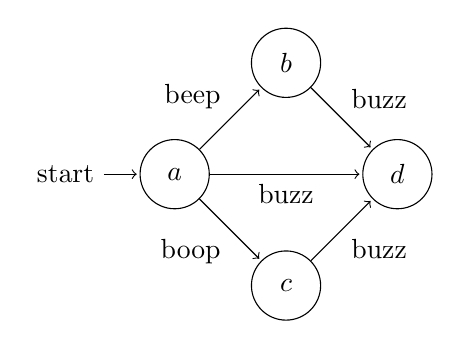
\begin{tikzpicture}[shorten >=1pt,node distance=2cm,on grid,auto]

  \node[state,initial]  (a)                    {$a$};
  \node[state]          (b) [above right=of a] {$b$};
  \node[state]          (c) [below right=of a] {$c$};
  \node[state]          (d) [below right=of b] {$d$};

  \path[->] (a)   edge              node        {beep} (b)
                  edge              node [swap] {boop} (c)
                  edge              node [swap] {buzz} (d)
            (b)   edge              node        {buzz} (d)
            (c)   edge              node [swap] {buzz} (d);
\end{tikzpicture}

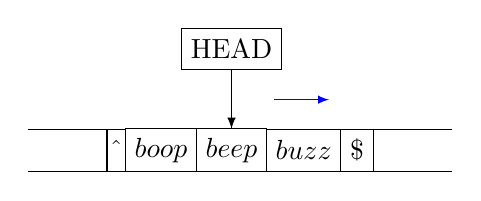
\begin{tikzpicture}[every node/.style={block},
        block/.style={minimum height=1.5em,outer sep=0pt,draw,rectangle,node distance=0pt}]
   \node (A) {$beep$};
   \node (B) [left=of A] {$boop$};
   \node (C) [left=of B] {$ \hat{} $};
   \node (D) [right=of A] {$buzz$};
   \node (E) [right=of D] {$\$ $};
   \node (F) [above = 0.75cm of A] {HEAD};
   \draw[-latex] (F) -- (A);
   \draw[-latex,blue] ($(F.east)!0.5!(A.east)$) -- ++(7mm,0);
   \draw (C.north west) -- ++(-1cm,0) (C.south west) -- ++ (-1cm,0) 
                 (E.north east) -- ++(1cm,0) (E.south east) -- ++ (1cm,0);
\end{tikzpicture}

\end{document}
